\documentclass[aspectratio=1610]{beamer}
\usepackage[utf8]{inputenc}
\usepackage[T1]{fontenc}
\usepackage[german]{babel}
\usepackage[useregional]{datetime2}
\usepackage[nameinlink]{cleveref}
\usepackage[section]{placeins}
\usepackage{xcolor}
\usepackage{graphicx}
\usepackage{csquotes}
\usepackage{amsmath} % for $\text{}$
\usepackage{enumitem}
\usepackage{abschluss}
\usepackage{algorithm}
\usepackage{algorithmicx}
\usepackage{algpseudocode}
\usepackage{listings}
\usepackage{bera}
\usepackage{pdfpages}
\usepackage{colortbl}
\usepackage{chronosys}

\colorlet{punct}{red!60!black}
\definecolor{background}{HTML}{EEEEEE}
\definecolor{delim}{RGB}{20,105,176}
\colorlet{numb}{magenta!60!black}
\lstdefinelanguage{json}{
    basicstyle=\normalfont\ttfamily,
    numbers=left,
    numberstyle=\scriptsize,
    stepnumber=1,
    numbersep=8pt,
    showstringspaces=false,
    breaklines=true,
    frame=lines,
    backgroundcolor=\color{background},
    literate=
     *{0}{{{\color{numb}0}}}{1}
      {1}{{{\color{numb}1}}}{1}
      {2}{{{\color{numb}2}}}{1}
      {3}{{{\color{numb}3}}}{1}
      {4}{{{\color{numb}4}}}{1}
      {5}{{{\color{numb}5}}}{1}
      {6}{{{\color{numb}6}}}{1}
      {7}{{{\color{numb}7}}}{1}
      {8}{{{\color{numb}8}}}{1}
      {9}{{{\color{numb}9}}}{1}
      {:}{{{\color{punct}{:}}}}{1}
      {,}{{{\color{punct}{,}}}}{1}
      {\{}{{{\color{delim}{\{}}}}{1}
      {\}}{{{\color{delim}{\}}}}}{1}
      {[}{{{\color{delim}{[}}}}{1}
      {]}{{{\color{delim}{]}}}}{1},
}

\setlist{nosep}

\newcommand\urlpart[2]{$\underbrace{\text{\texttt{#1}}}{\text{#2}}$}
\raggedbottom
\crefname{figure}{Abb}{Abb}

\newcommand\producttitle{treff.}
\hypersetup{
	pdftitle={Qualitätssicherungsphase: \producttitle},
	bookmarks=true,
}

% header & footer
\usepackage{scrlayer-scrpage}
%\lofoot{\today}
%\refoot{\today}
\pagestyle{scrheadings}

\title{
\includegraphics[width = 50mm]{images/logo_crop.png}}
\subtitle{\huge Abschlusspräsentation}
\author{Lukas Dippon
	\and Jens Kienle
	\and Matthias Noll
    \\Fabian Röpke
	\and Tim Schmidt
	\and Simon Vögele}

\begin{document}

	\begin{frame}[plain]
	\maketitle
	\end{frame}

%%%%%%%% Idee/Vision %%%%%%%%%%

	\begin{frame}[plain]
      \frametitle{\textbf{Aufgabenstellung}}
      \begin{itemize}
        \item[--] Entwicklung einer Android App
        \item[--] Verwendung einer Client-Server Architektur
        \item[--] Inspiration durch "Go-App"
        \item[--] App zum Koordinieren kleiner Personenkreise
        \item[--] Keine closed source dependencies
        \item[--] Kein Ungewolltes Tracking
        \item[--] Kein Social Network
      \end{itemize}
  \end{frame}

  \begin{frame}[plain]
      \frametitle{\textbf{Datenmodell}}
      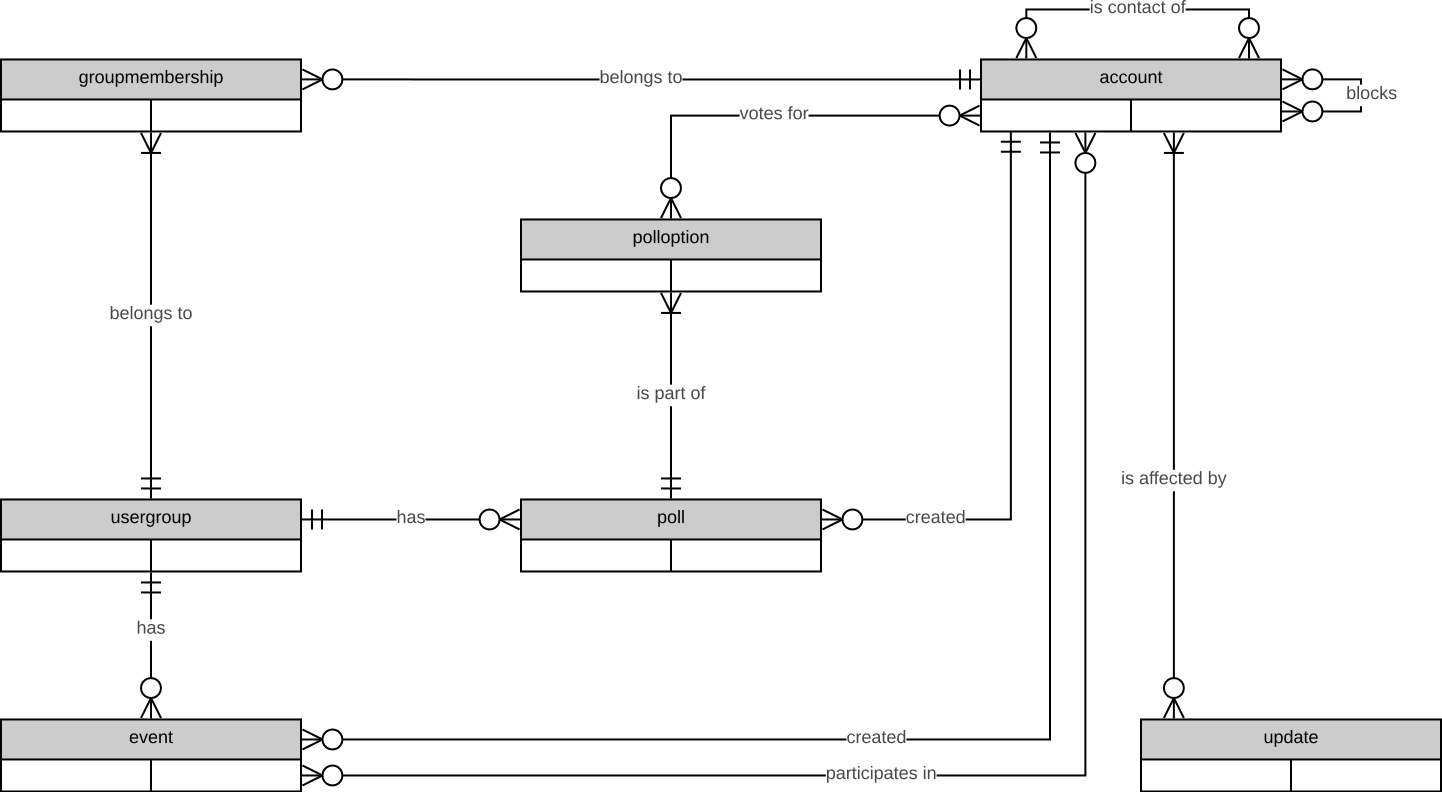
\includegraphics[width = \columnwidth - 30pt]
        {images/erd.png}
      %TODO ggf auf anderem Bildschirm zeitgleich mit der Folie davor?
      %TODO andere Darstellung
  \end{frame}

%%%%%%%% Umsetzung %%%%%%%%%%

  \begin{frame}[plain]
      \frametitle{\textbf{Arbeitsweise - Arbeitsaufteilung}}
      \begin{itemize}
          \setlength\itemsep{0.3em}
          \item[--] 3 Personen für den Klient
              \begin{itemize}
                  \item[--] Fabian
                  \item[--] Lukas
                  \item[--] Matthias
              \end{itemize}
          \item[--] 3 Personen für den Server
              \begin{itemize}
                  \item[--] Jens
                  \item[--] Simon
                  \item[--] Tim
              \end{itemize}
      \end{itemize}
  \end{frame}

  \begin{frame}[plain]
      \frametitle{\textbf{Arbeitsweise - Tools}}
      \begin{minipage}{0.45\textwidth}
        \begin{itemize}
          \item[--] GitHub
          \item[--] LaTeX
          \item[--] IntelliJ/AndroidStudio
          \item[--] Kanban board \& Etherpad
          \item[--] PlantUML
        \end{itemize}
      \end{minipage}
      \begin{minipage}{0.45\textwidth}
        
\includegraphics[width = \columnwidth - 30pt]
          {images/tools.png}
      \end{minipage}
  \end{frame}

  \begin{frame}[plain]
      \frametitle{\textbf{Arbeitsweise - Kommunikation}}
      \begin{minipage}{0.45\textwidth}
        \begin{itemize}
          \item[--] Telegram
          \item[--] Discord \& TS
          \item[--] Persönliche Treffen \\ v.a. zwischen Vorlesungen
        \end{itemize}
      \end{minipage}
      \begin{minipage}{0.45\textwidth}
        
\includegraphics[width = \columnwidth - 30pt]
          {images/meet-im-voip.png}
      \end{minipage}
  \end{frame}

  \begin{frame}[plain]
      \frametitle{\textbf{Interessante Stellen - Server}}
      %TODO Locking, rdm Updates
  \end{frame}

  \begin{frame}[plain]
      \frametitle{\textbf{Interessante Stellen - Client}}
      %TODO osmdroid (clustering etc)
  \end{frame}

  \begin{frame}[plain]
      \frametitle{\textbf{Probleme}}
      \begin{itemize}
        \item[--] Arbeitsaufwand unterschätzt
        %TODO LoC-Graph auf anderem Bildschirm
        \item[--] Teilweise schlechtes Zeitmanagement
        %TODO Phasengrenzen in LoC-Graph einblenden
        \item[--] Zu wenig Leute beim Client
        \item[--] Aufteilung in Teams => mangelnde Kommunikation
        \item[--] Zu wenig Gedanken über Implementierung im Entwurf
        \item[--] Zu wenig Gedanken über Qualitätssicherung bei der Implementierung
      \end{itemize}
  \end{frame}

%%%%%%%% Ergebnis %%%%%%%%%%

  \begin{frame}[plain]
      \frametitle{\textbf{Demo}}

  \end{frame}

  \begin{frame}[plain]
      \frametitle{\textbf{Erweiterungsmöglichkeiten}}
        \begin{itemize}
          \item[--] Abstimmungen
          \item[--] Gruppenrollen und -rechte
          \item[--] Detaillierte Innenraumkarten
          \item[--] Stummschalten
          \item[--] Zeitplan für Positionsübertragung
          \item[--] Passwortzurücksetzung
          \item[--] Profil- und Gruppenbilder
          %TODO Bilder auf dem anderen Bildschirm?
        \end{itemize}
  \end{frame}

\end{document}
